\chapter{Definicja Problemu}

\section*{Streszczenie}
W poniższym rozdziale zostanie zaprezentowany problem, który usiłują rozwiązać systemy bazodanowe opisane w niniejszej pracy.
Przedstawione zostaną także sposoby radzenia sobie z tym problemem przy zastosowaniu relacyjnych baz danych.

\section{Wstęp}
Popularyzacja dostępu do internetu przyczyniła się w ostatnich latach do  powstania licznych serwisów, które mogą się pochwalić dziesiątkami, a nawet setkami milionów odwiedzin dziennie. 
Twórcy serwisów takich jak Facebook, Twitter czy Google zostali postawieni przed problemem stworzenia rozproszonej architektury bazodanowej, która zapewni horyzontalną skalowalność przy równoczesnym zachowaniu wysokiej dostępności. 
Ze względu na występujący jeszcze kilka lat temu brak takich rozwiązań na rynku firmy te były zmuszone do implementacji tego typu baz na własne potrzeby. 
Ostatnimi laty jednak sytuacja zaczęła ulegać zmianie: produkty wytworzone na wewnętrzny użytek zostają upubliczniane na licencjach Open Source, dzięki czemu obecnie mamy już dostęp do przynajmniej kilkunastu rozwiązań umożliwiających dostęp do peta-bajtów danych rozproszonych na tysiącach serwerów.

\section{Skalowalność}
Niniejsza praca stawia przed sobą zadanie wprowadzenia czytelnika w świat wysoce skalowalnych systemów bazodanowych.
Aby jednak tego dokonać musimy najpierw przedstawić, czym jest skalowalność w rozumieniu autora i jakiego typu skalowalnością będziemy się zajmować.

Wyobraźmy sobie aplikację internetową, na przykład stronę społecznościową taką jak Nasza Klasa czy Facebook.
Aplikacje takie jak ta początkowo mają tysiące użytkowników, a gdy odniosą sukces, liczba ta może wzrosnąć do dziesiątek czy nawet setek milionów.
Ponadto aplikacje te podlegają ciągłemu rozwojowi przez wiele lat, co bardzo często pociąga za sobą konieczność wprowadzania zmian w schemacie bazy, a także niejednokrotnie dokonywania migracji danych.

System bazodanowy jest skalowalny w rozumieniu tej pracy, jeżeli koszty jego utrzymania wzrastają co najwyżej liniowo wraz ze wzrostem liczby użytkowników aplikacji. 
Warunkiem koniecznym jest także to, aby czas potrzebny na wykonanie operacji na rzecz użytkownika aplikacji (zapisy, odczyty), nie degradował się znacznie wraz ze wzrostem ilości danych, którymi system zarządza.

\section{Problemy z tradycyjnymi rozwiązaniami}
Dotychczas najczęściej stosowanym rozwiązaniem problemów skalowalności było zastosowanie bazy danych takiej jak MySQL połączonej z Memcached jako przechowywany w pamięci operacyjnej, rozproszony cache\cite{highscalability-mysql-end-of-an-era}.
Opiszmy pokrótce, jak takie skalowanie aplikacji w uproszczeniu wygląda.

\subsection{Replikacja}
Początkowo cała baza danych mieści się na jednej maszynie i jest w stanie poradzić sobie ze wszystkimi operacjami odczytu i zapisu jakich dokonuje aplikacja.
Wraz ze wzrostem liczby użytkowników serwer zaczyna docierać do granic swojej przepustowości. 
Ponieważ aplikacje internetowe wykonują zazwyczaj dużo więcej odczytów niż zapisów, dodajemy stopniowo kilka kolejnych serwerów replikowanych w konfiguracji master-slave, zwiększając w ten sposób liczbę równoczesnych odczytów, jednak nie zwiększając (a nawet zmniejszając) liczby możliwych zapisów.
Alternatywą jest dodawanie kolejnych serwerów w konfiguracji master-master, która jest zazwyczaj trudniejsza do poprawnego skonfigurowania, ale za to w przypadku gdy jeden z serwerów master zawiedzie, inny z łatwością przejmie jego rolę.

\missingfigure{replikacje master-slave}

Warto jednak zwrócić uwagę, na to jak szybko takie rozwiązanie się degraduje.
Załóżmy, że początkowo serwer \emph{master} jest obciążony w 50\% zapisami.
Oznacza to, że każdy z węzłów \emph{slave} musi także poświęcić 50\% zasobów na radzenie sobie z replikacją zapisów\footnote{Zakładam, że wszystkie serwery są identyczne}, a resztę może poświęcić na przetwarzanie odczytów.
Wraz ze wzrostem obciążenia serwera \emph{master}, serwery \emph{slave} muszą coraz więcej zasobów poświęcać na replikację zapisów, co zmniejsza ogólną przepustowość systemu.
Ponadto problemem może być także to, że niektóre systemy baz danych, tak jak, np. MySQL dokonują replikacji asynchronicznie.
Powoduje to, że po dokonaniu operacji zapisu, odczyt może zwrócić wartość niezgodą z zapisaną.
Wymaga to dodatkowej pracy ze strony programisty\cite{zaitsev-scaling-mysql}.

\subsection{Partycjonowanie}
Kiedy oczywiste staje się, że nasz serwer nie jest w stanie sobie poradzić z obciążeniem wynikającym z zapisów, mamy dwie drogi do wyboru: wymienić maszynę na mocniejszą, albo zacząć przetrzymywać tylko część danych na pojedynczym serwerze.
Pierwsza opcja, nazywana \emph{skalowaniem wzwyż}, ma pewne zalety: nie wymaga zmian w aplikacji i jej nie komplikuje.
Wadą tego rozwiązania jest jednak cena w porównaniu do możliwości.
Cytując za artykułem na blogu \emph{Coding Horror}\cite{codinghorror-scaling-up-vs-out}: za cenę stu tysięcy dolarów możemy albo kupić jeden potężny serwer z 32 procesorami, 512GB RAM i 4TB przestrzeni dyskowej, albo 83 mniejsze serwery posiadające łącznie 332 rdzenie, 664GB RAM i 40,5TB przestrzeni dyskowej.
Oczywiście nie można w ten sposób skalować aplikacji wzwyż w nieskończoność, ale warto pamiętać, że tylko nieliczne strony mogą konkurować rozmiarami z takimi gigantami jak Facebook.
Większość aplikacji nigdy nie wyrośnie ponad rozmiar, w którym superkomputer nie wystarcza już do utrzymania ich obciążenia.

\begin{figure}[!ht]
 \centering
 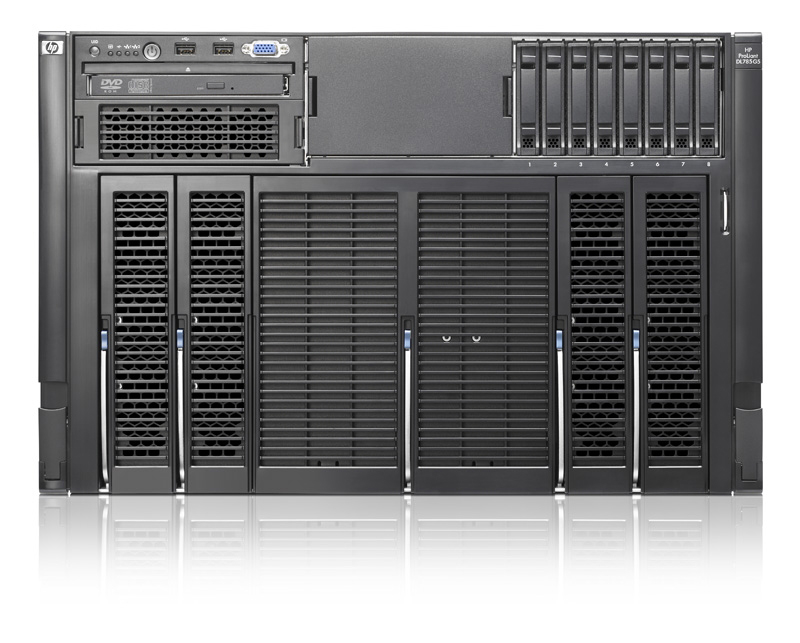
\includegraphics[width=0.75\textwidth]{chapters/definicja_problemu/hp-proliant-dl785.jpg}
 % hp-proliant-dl785.jpg: 400x400 pixel, 100dpi, 10.16x10.16 cm, bb=0 0 288 288
 \caption{HP ProLiant DL785 G5}
 \label{fig:superkomputer}
\end{figure}

Z drugiej strony mamy partycjonowanie danych, czyli \emph{skalowanie aplikacji wszerz}.
W tym rozwiązaniu wraz ze wzrostem liczby użytkowników zamiast wymieniać serwer na większy i mocniejszy dodajemy kolejne maszyny.
Nie możemy jednak całości bazy danych przechowywać na każdym z serwerów - problemy z tym związane zostały opisane powyżej.
W związku z tym, dokonuje się podziału danych (partycjonowania) poziomego, pionowego albo obu równocześnie.

Kiedy mowa o pojedynczej bazie danych, horyzontalne partycjonowanie oznacza, że rzędy na podstawie jakiegoś kryterium trafiają do różnych tabel.
Dla przykładu: tabela użytkowników może być podzielona w taki sposób, że użytkownicy z Polski trafiają do tabeli \verb=polish_users=, natomiast użytkownicy z Niemiec do tabeli \verb=german_users=.
Tego rodzaju partycjonowania dokonuje się zazwyczaj w celu zwiększenia wydajności i niektóre bazy danych (w tym MySQL\footnote{http://dev.mysql.com/tech-resources/articles/performance-partitioning.html}) pozwalają na definiowanie partycjonowania w schemacie bazy danych.
W przypadku rozproszonych baz danych, mówimy zamiennie o partycjonowaniu horyzontalnym bądź shardowaniu (ang. \emph{sharding}).
Różni się ono od partycjonowania poziomego dla pojedynczej bazy tym, że dane zamiast trafiać do różnych tabel, trafiają do tej samej tabeli, ale na różne węzły bazy danych.

\missingfigure{shardownie}

Partycjonowanie pionowe (wertykalne) podobnie ma dwa znaczenia w zależności od kontekstu.
Dla pojedynczej bazy polega ono na podziale tabel na mniejsze (zawierające tylko część kolumn).
Przypomina to normalizację bazy, ale dzielimy także już znormalizowane tabele, np. po to aby aby część kolumn umieścić na innym dysku, albo aby oddzielić częściej odczytywane dane od rzadziej odczytywanych.
W rozproszonym systemie partycjonowanie pionowe oznacza, że nie połączone ze sobą tabele mogą być umieszczone na różnych węzłach bazy danych.
W ten sposób zapis do jednej tabeli nie obciąża dwóch, tylko jeden serwer.
Oczywiście bardzo często nie jest możliwe znalezienie tabel, które nie są za sobą połączone pośrednio lub bezpośrednio.
Dlatego często takie partycjonowanie wymaga zduplikowania części tabel na obu węzłach.

Opisane wyżej formy partycjonowania systemów rozproszonych najczęściej muszą być obsługiwane przez warstwę aplikacji.
Z tego względu praktycznie niemożliwe jest zapewnienie transakcyjności pomiędzy poszczególnymi węzłami.
Kosztowne i trudne są także operacje joinowania pomiędzy serwerami.

\subsection{Memcached}
\todo{tu skończyłem}

\section{NoSQL}
Powszechny i darmowy dostęp do produktów bazodanowych obiecujących wysoką skalowalność zaowocował powstaniem ruchu określanego popularnie mianem NoSQL (\emph{Not only SQL} - nie tylko SQL). 
Nazwa ta bierze się stąd, że większość nowych produktów bazodanowych stworzonych z myślą o wysokiej skalowalności nie dysponuje możliwością zadawania zapytań w języku SQL. 
Ruch ten jest zainteresowany problematyką dużych i bardzo dużych serwisów internetowych, które ze względów wydajnościowych nie stać na wykorzystywanie tradycyjnych silników bazodanowych z transakcjami i łączeniem tabel w zapytaniach.

W literaturze trudno znaleźć nazwę problemu, który próbuje rozwiązać ruch NoSQL. 
W artykule \cite{monash-db-hvsp} autor sugeruje nazwę HVSP (ang. \emph{High Volume Simple Processing}). 
Sugerowane wyróżniki problemu to:
\begin{itemize}
 \item Wielu równocześnie korzystających z bazy użytkowników, dokonujących zarówno odczytów, jak i zapisów.
 \item Operacje wykonywane przez użytkowników są nieskomplikowane, bez transakcji, łączenia tabel, czy operacji grupujących.
\end{itemize}

Dotychczas popularnym rozwiązaniem było stosowanie zdenormalizowanych, horyzontalnie dzielonych (ang. \emph{sharded}) i replikowanych baz (np. MySQL) wspartych przez przechowywany w pamięci RAM serwerów cache (zazwyczaj Memcached). 
Produkty NoSQL zazwyczaj idą o krok dalej całkowicie pozbywając się transakcji i joinów, a często także sztywnego schematu bazy.

\section{Cel pracy}
Praca dyplomowa, której konspekt niniejszym przedstawiam, ma na celu opisanie dostępnych na rynku rozwiązań NoSQL, zwracając uwagę na szczególne właściwości i możliwości zastosowania poszczególnych produktów, jak również ich dojrzałości, tempa ich rozwoju, oceny aktywności ich użytkowników i ekosystemu narzędzi z nimi związanych. 
Elementem tego porównania będzie także zbudowanie frameworku do przeprowadzania testów na części zaprezentowanych produktów, zróżnicowanych pod względem klas tych rozwiązań (osobno dla \emph{document oriented} \emph{key-value stores}, \emph{table oriented}, \emph{graph oriented}).
Ponieważ każde narzędzie dysponuje własną nomenklaturą konieczne będzie także wprowadzenie jednolitego nazewnictwa, które ułatwi zrozumienie, oraz porównanie opisanych produktów.

Porównanie takie uważam za wartościowe, ze względu na to, iż będzie najprawdopodobniej jednym z pierwszych obszernych porównań produktów NoSQL, a możliwe że pierwszym takim napisanym w języku polskim.
